\section{Tests on the MeerKAT LMC observation}\label{results}
For algorithmic testing


	
\begin{figure}[h]
	\centering
	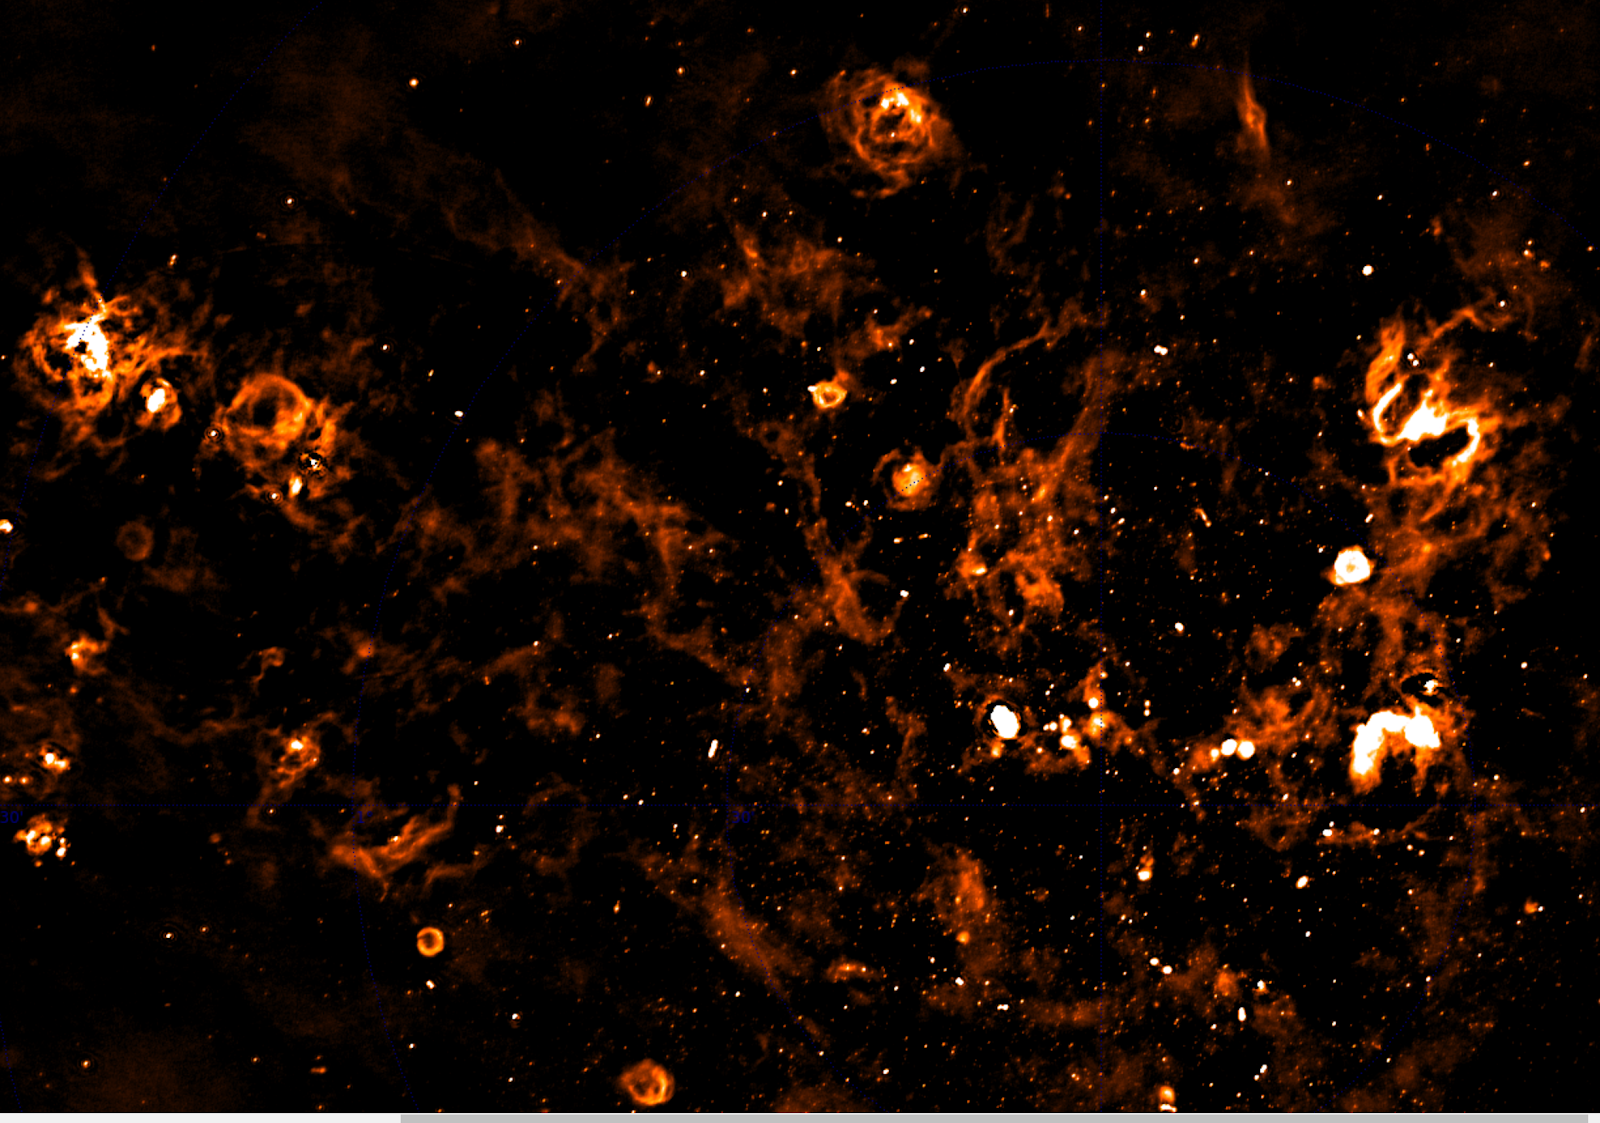
\includegraphics[width=0.80\linewidth]{./chapters/10.results/LMC/meerkat.png}
	\caption{Radio interferometer system}
	\label{results:radio}
\end{figure}



\subsection{Comparison with CLEAN reconstruction}

\subsection{GPU Acceleration}

\subsection{Distributed coordinate descent}




We are in the realm of convolution. Remember that a convolution in image space is a multiplication in fourier space.
We can multiply

\subsection{Wall clock time}
\begin{figure}[h]
	\centering
	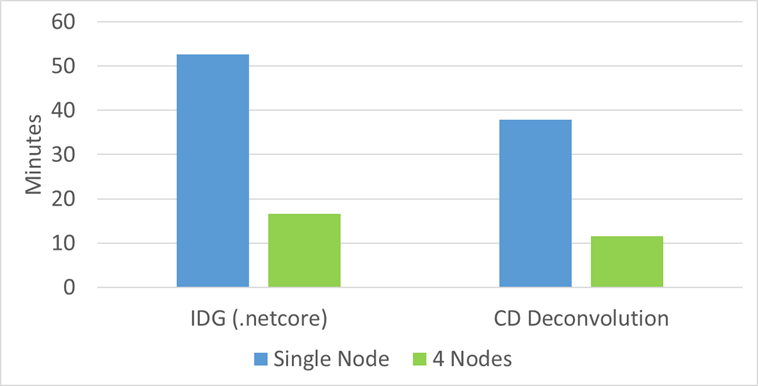
\includegraphics[width=0.80\linewidth]{./chapters/10.results/wall-clock-time.png}
	\caption{Wall-clock time of the distributed reconstruction}
	\label{results:time:fig}
\end{figure}


\subsection{Validity of gradient approximation} \label{results:gradients}